\documentclass[11pt]{article}
\usepackage[margin=1in]{geometry}
\usepackage{amsmath,amssymb,amsthm,graphicx,booktabs}
\graphicspath{{../sims/out/}}
\setlength{\parindent}{0pt}\setlength{\parskip}{6pt}
\newtheorem{proposition}{Proposition}
\newtheorem{corollary}{Corollary}
\theoremstyle{remark}\newtheorem*{remark}{Remark}
\newcommand{\E}{\mathbb{E}}
\newcommand{\Var}{\operatorname{Var}}
\newcommand{\Cov}{\operatorname{Cov}}
\newcommand{\tr}{\operatorname{tr}}
\title{An Exact, Distribution-Free SURE for Shrinkage Toward $\nu I$}
\author{Jack Wang}
\date{October 26, 2026}
\begin{document}
\maketitle
\vspace{-2em}

\section{Setup}
Let $X_1,\dots,X_T\in\mathbb{R}^p$ be i.i.d.\ with mean zero (known), covariance $\Sigma$ and
$\E\|X\|^4<\infty$. No distributional form is assumed. Let
\[
S=\frac1T\sum_{t=1}^T X_tX_t^\top,\qquad F=\nu I,\quad \nu=\frac{\tr S}{p},\qquad
\hat\Sigma_\alpha=\alpha F+(1-\alpha)S .
\]
Because the mean is known, $\E S=\Sigma$, so Lemma~1 of Yi and Zou (2013) applies (see
\texttt{sure\_derivation.pdf}):
\begin{equation}\label{eq:risk}
R(\alpha)=\E\|\hat\Sigma_\alpha-\Sigma\|_F^2=\alpha^2 D+(1-2\alpha)V+2\alpha C,
\end{equation}
\[
D=\E\|F-S\|_F^2,\qquad V=\sum_{i,j}\Var(s_{ij}),\qquad C=\sum_{i,j}\Cov(f_{ij},s_{ij}).
\]
Define the statistics
\[
\hat M=\frac1T\sum_t\|X_t\|^4,\qquad
\hat U_2=\frac{1}{T(T-1)}\sum_{t\neq u}(X_t^\top X_u)^2,\qquad
\hat U_3=\frac{1}{T(T-1)}\sum_{t\neq u}\|X_t\|^2\|X_u\|^2 .
\]
They are cheap to compute because
$\sum_{t,u}(X_t^\top X_u)^2=T^2\tr(S^2)$ and $\sum_{t,u}\|X_t\|^2\|X_u\|^2=T^2(\tr S)^2$, so
\[
\hat U_2=\frac{T\tr(S^2)-\hat M}{T-1},\qquad \hat U_3=\frac{T(\tr S)^2-\hat M}{T-1}.
\]

\section{Results}

\begin{proposition}[Unbiased estimates of $V$ and $C$]\label{prop:unbiased}
Under the setup above,
\[
\hat V=\frac{\hat M-\hat U_2}{T},\qquad \hat C=\frac{\hat M-\hat U_3}{pT}
\]
satisfy $\E\hat V=V$ and $\E\hat C=C$.
\end{proposition}

\begin{proof}
\emph{The term $V$.} The entry $s_{ij}=\frac1T\sum_t x_{ti}x_{tj}$ is an average of i.i.d.\ terms, so
$\Var(s_{ij})=\frac1T\big(\E[x_i^2x_j^2]-\sigma_{ij}^2\big)$. Summing over $i,j$, and using
$\sum_{i,j}x_i^2x_j^2=\|X\|^4$ and $\sum_{i,j}\sigma_{ij}^2=\tr(\Sigma^2)$,
\[
V=\frac{\E\|X\|^4-\tr(\Sigma^2)}{T}.
\]
$\hat M$ is a sample mean of $\|X_t\|^4$, so $\E\hat M=\E\|X\|^4$. For $t\neq u$, independence gives
$\E(X_t^\top X_u)^2=\E\,\tr(X_tX_t^\top X_uX_u^\top)=\tr(\Sigma\Sigma)$, so $\E\hat U_2=\tr(\Sigma^2)$.

\emph{The term $C$.} Since $f_{ij}=\nu\,\delta_{ij}$,
\[
C=\sum_i\Cov(\nu,s_{ii})=\frac1p\Cov\Big(\tr S,\sum_i s_{ii}\Big)=\frac1p\Var(\tr S).
\]
$\tr S=\frac1T\sum_t\|X_t\|^2$ is an i.i.d.\ average, so
$\Var(\tr S)=\frac1T\big(\E\|X\|^4-(\tr\Sigma)^2\big)$. For $t\neq u$,
$\E\|X_t\|^2\|X_u\|^2=(\tr\Sigma)^2$, so $\E\hat U_3=(\tr\Sigma)^2$.
\end{proof}

\begin{corollary}[Exact SURE]\label{cor:sure}
For every fixed $\alpha$,
\[
\mathrm{SURE}(\alpha)=\alpha^2\|F-S\|_F^2+(1-2\alpha)\hat V+2\alpha\hat C
\]
satisfies $\E\,\mathrm{SURE}(\alpha)=R(\alpha)$. It is minimized at
\[
\hat\alpha_{\mathrm{SURE}}=\frac{\hat V-\hat C}{\|F-S\|_F^2},
\]
which we clip to $[0,1]$.
\end{corollary}
The observed $\|F-S\|_F^2$ is trivially unbiased for $D$, and SURE is linear in
$(\|F-S\|^2,\hat V,\hat C)$. The minimizer $\hat\alpha_{\mathrm{SURE}}$ is a ratio of estimates, so it is
\emph{not} unbiased for $\alpha^*$. Unbiasedness holds for the risk curve, not for its argmin.

\begin{proposition}[When shrinkage reduces risk]\label{prop:reduce}
Let $\alpha^*=(V-C)/D$. Then $\alpha^*\ge 0$, and
\[
R(\alpha)<R(0)\iff 0<\alpha<2\alpha^* .
\]
\end{proposition}

\begin{proof}
From \eqref{eq:risk}, $R(\alpha)-R(0)=\alpha^2D-2\alpha(V-C)=\alpha D(\alpha-2\alpha^*)$. Since
$D>0$, this is negative exactly when $\alpha$ lies strictly between $0$ and $2\alpha^*$.

To see that $V\ge C$, apply Cauchy--Schwarz to $\tr S=\sum_i s_{ii}$:
$\Var(\tr S)\le\big(\sum_i\sqrt{\Var s_{ii}}\big)^2\le p\sum_i\Var(s_{ii})$. Hence
$C=\Var(\tr S)/p\le\sum_i\Var(s_{ii})\le V$.
\end{proof}

The sample analogue is that $\mathrm{SURE}(\alpha)<\mathrm{SURE}(0)$ if and only if
$0<\alpha<2\hat\alpha_{\mathrm{SURE}}$. This is an exact algebraic statement about the estimated curve.
The statement about the true risk uses $\alpha^*$, not $\hat\alpha$. This corrects the version in the
progress log, which stated the condition with $\hat\alpha$.

\begin{proposition}[Ledoit--Wolf is SURE minus two finite-sample terms]\label{prop:lw}
The LW (2004) intensity toward $\nu I$ (eq.~13 in Chen et al., 2010) is
\[
\hat\rho_{\mathrm{LW}}=\frac{\sum_t\|X_tX_t^\top-S\|_F^2}{T^2\,\|F-S\|_F^2}
=\frac{\tfrac{T-1}{T}\,\hat V}{\|F-S\|_F^2},
\qquad\text{whereas}\qquad
\hat\alpha_{\mathrm{SURE}}=\frac{\hat V-\hat C}{\|F-S\|_F^2}.
\]
\end{proposition}

\begin{proof}
Expanding the square,
$\sum_t\|X_tX_t^\top-S\|^2=\sum_t\|X_t\|^4-2T\tr(S^2)+T\tr(S^2)=T(\hat M-\tr S^2)$.
Substituting $\tr S^2=\big(\hat M+(T-1)\hat U_2\big)/T$ gives $T\cdot\frac{T-1}{T}(\hat M-\hat U_2)$.
Dividing by $T^2$ yields $\frac{T-1}{T}\hat V$. The denominators agree because
$\tr(S^2)-(\tr S)^2/p=\|S-\nu I\|_F^2$.
\end{proof}

So LW and SURE share the denominator. They differ only in the numerator: LW multiplies $\hat V$ by
$(T-1)/T$ and drops $\hat C=\widehat{\Var}(\tr S)/p$. Both differences vanish as $T\to\infty$, which is
why LW is consistent. In small samples the $(T-1)/T$ factor dominates and LW under-shrinks
relative to the oracle, as the simulation shows. (The script confirms the identity to 10 digits.)

\begin{remark}[Gaussian consistency check]
Under Gaussianity, $\E\|X\|^4=(\tr\Sigma)^2+2\tr(\Sigma^2)$. Then
$V=\big(\tr\Sigma^2+\tr^2\Sigma\big)/T$, $C=2\tr\Sigma^2/(pT)$, and
$D=\tr\Sigma^2+V-\tr^2\Sigma/p-C$. Substituting,
\[
\alpha^*=\frac{(1-2/p)\tr\Sigma^2+\tr^2\Sigma}{(T+1-2/p)\tr\Sigma^2+(1-T/p)\tr^2\Sigma},
\]
which is exactly the Gaussian oracle in eq.~(7) of Chen et al.\ (2010). The decomposition
\eqref{eq:risk} therefore reproduces their oracle as a special case. Outside the Gaussian family,
the kurtosis enters through $\E\|X\|^4$, and $\hat M$ estimates it directly.
\end{remark}

\section{Simulation}
Code: \texttt{sims/sure\_sim.py} (seed 20261026, about 20\,s). $\Sigma$ is AR(1) with $r=0.5$ and $p=100$.
The data are Gaussian or multivariate $t_{10}$ rescaled to covariance $\Sigma$. We use 10 degrees of
freedom so that $\hat V$ and $\hat C$ have finite variance, which needs finite 8th moments.
The true $V,C,D$ are in closed form, using $\E\|X\|^4=\kappa\,(\tr^2\Sigma+2\tr\Sigma^2)$ with
$\kappa=1$ (Gaussian) or $\kappa=(\nu-2)/(\nu-4)$ ($t_\nu$).

\subsection*{Unbiasedness (Proposition~\ref{prop:unbiased})}
20{,}000 replications per row. Every mean is within about 1.3 Monte Carlo standard errors of the truth.

\begin{center}\small
\begin{tabular}{lrrrrrrrr}
\toprule
data & $p$ & $T$ & $V$ & mean $\hat V$ & s.e. & $C$ & mean $\hat C$ & s.e.\\
\midrule
Gaussian & 10 & 5 & 23.156 & 23.223 & 0.094 & 0.6311 & 0.6330 & 0.0050\\
Gaussian & 50 & 10 & 258.244 & 258.455 & 0.306 & 0.3298 & 0.3286 & 0.0013\\
Gaussian & 100 & 40 & 254.144 & 254.173 & 0.105 & 0.0829 & 0.0828 & 0.0001\\
$t_{10}$ & 10 & 5 & 31.926 & 32.142 & 0.338 & 1.5082 & 1.5114 & 0.0275\\
$t_{10}$ & 50 & 10 & 347.074 & 345.813 & 1.754 & 2.1064 & 2.0800 & 0.0247\\
$t_{10}$ & 100 & 40 & 340.241 & 339.157 & 0.861 & 0.9439 & 0.9386 & 0.0061\\
\bottomrule
\end{tabular}
\end{center}

\subsection*{SURE curve against the true risk (Goal 2)}
Figure~\ref{fig:curves} has $p=100$ and $T=20$. The average of 4{,}000 SURE curves matches the
closed-form $R(\alpha)$ to within 0.2\% (Gaussian) and 0.1\% ($t_{10}$) of $\max R$. A direct Monte Carlo
of the loss lies on the same line. Individual curves (grey) are noisy, especially under heavy tails,
but their minimizers cluster near $\alpha^*$.

\begin{figure}[h]\centering
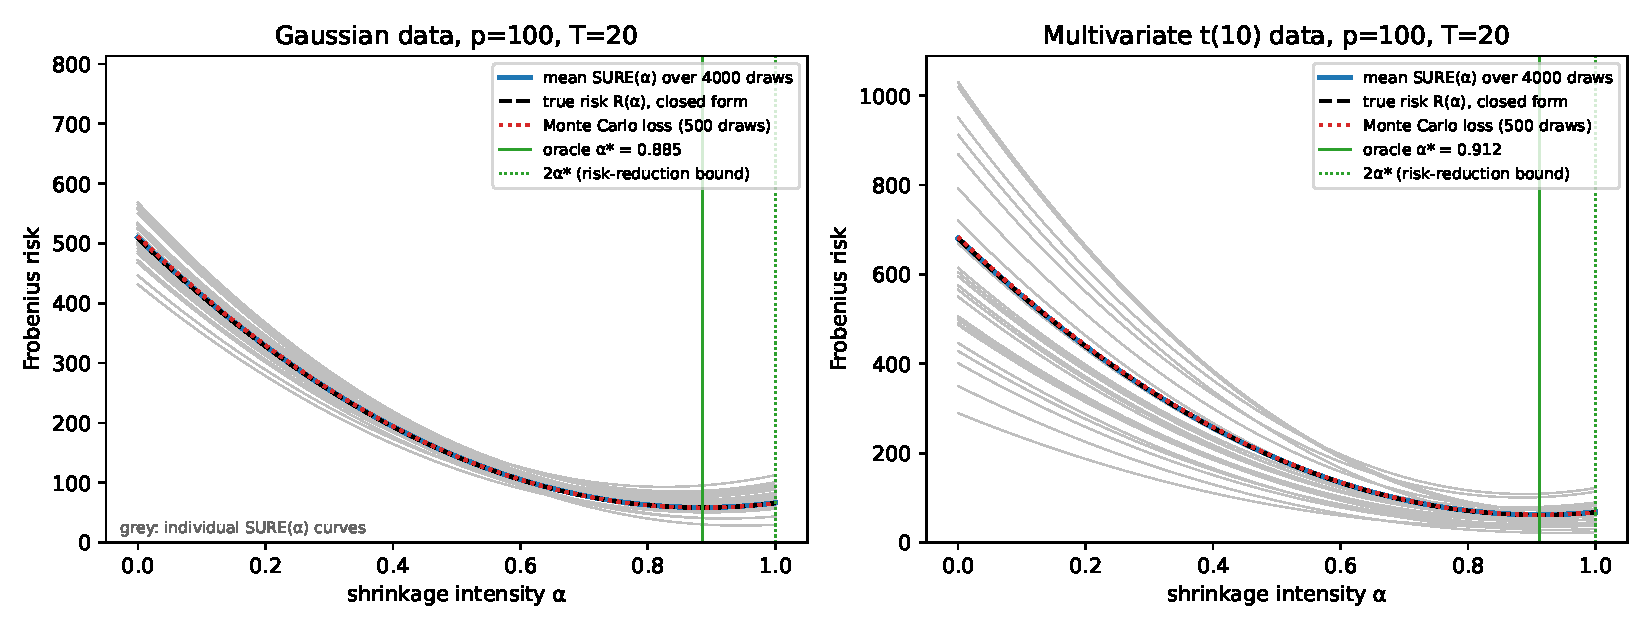
\includegraphics[width=\linewidth]{fig_sure_vs_risk.pdf}
\caption{SURE$(\alpha)$ against the true Frobenius risk. Solid green: $\alpha^*$. Dotted green: $2\alpha^*$,
the upper end of the risk-reduction interval (Prop.~\ref{prop:reduce}), here clipped at 1.}
\label{fig:curves}
\end{figure}

\subsection*{Comparison with LW, RBLW and OAS (Goal 4)}
2{,}000 replications per $T$, with $p=100$. ``Oracle'' uses the fixed $\alpha^*$ computed from the true $\Sigma$.

\begin{figure}[h]\centering
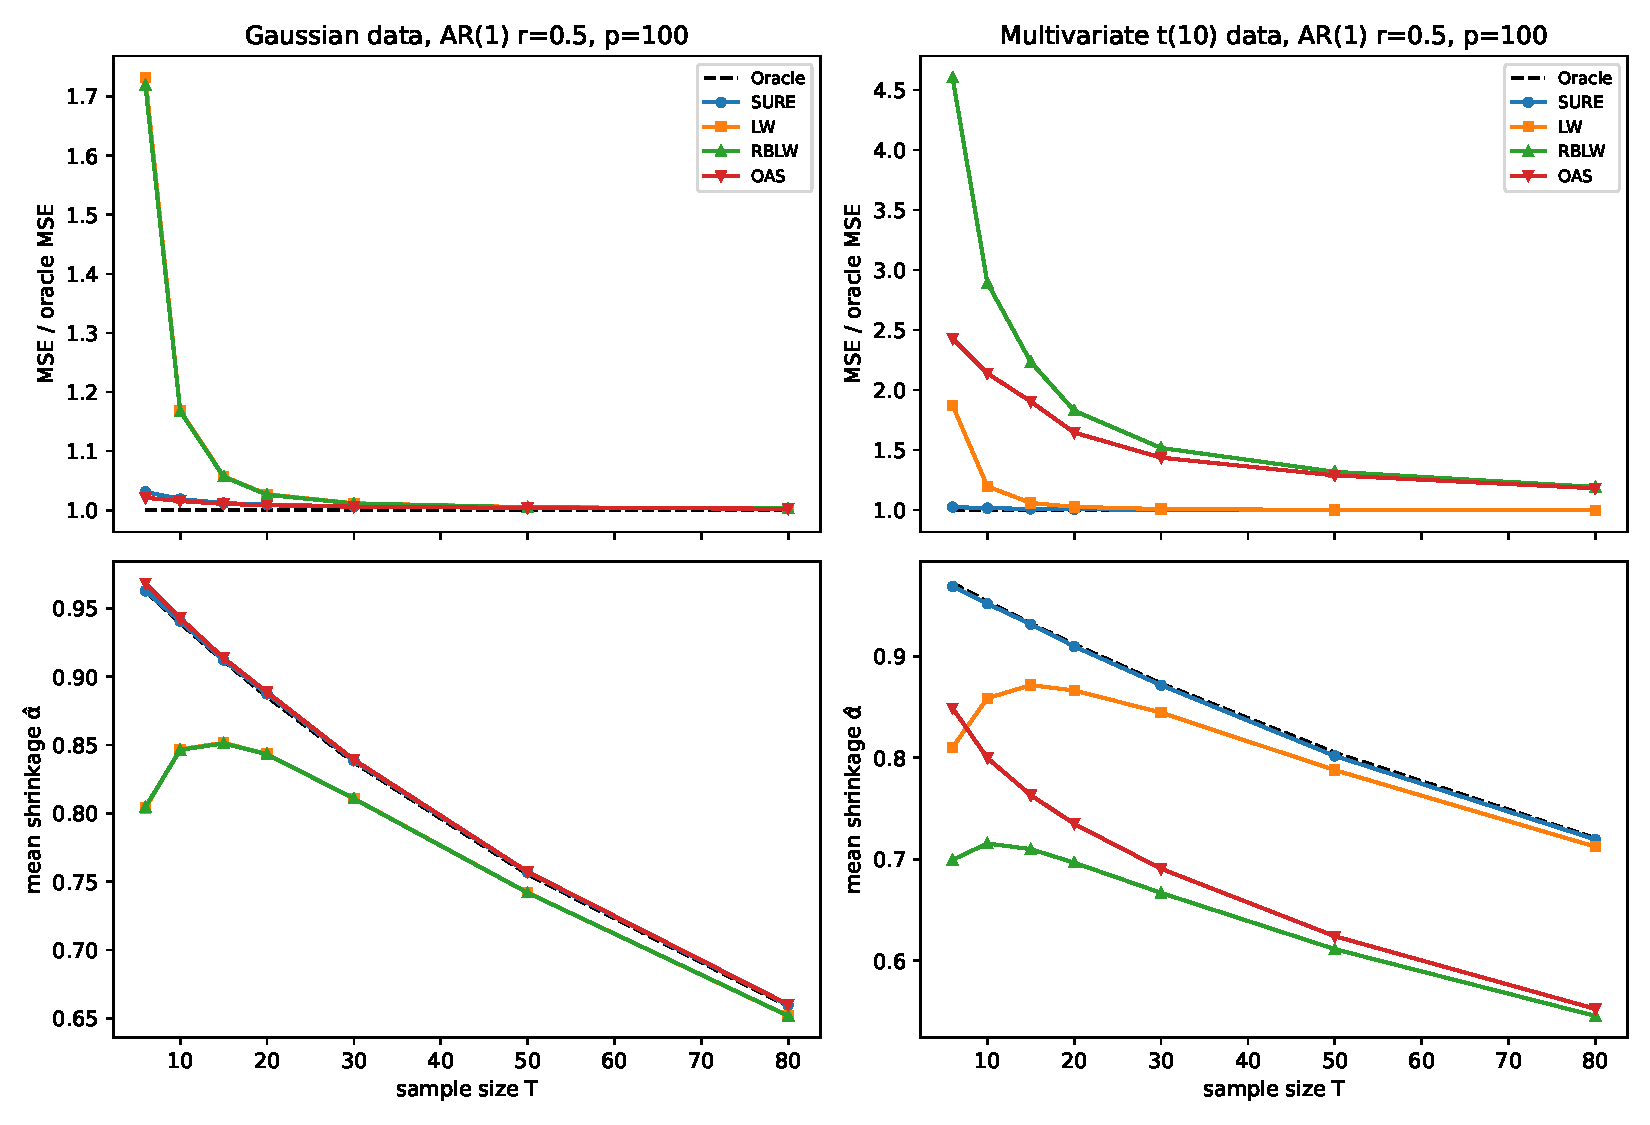
\includegraphics[width=\linewidth]{fig_compare.pdf}
\caption{Top: Frobenius MSE relative to the oracle. Bottom: mean shrinkage intensity.}
\label{fig:compare}
\end{figure}

\begin{itemize}
\item \textbf{Gaussian data.} SURE and OAS are indistinguishable and stay within 3\% of the oracle at every $T$.
LW and RBLW under-shrink badly when $T$ is small ($\hat\rho\approx0.80$ against $\alpha^*=0.96$ at $T=6$),
giving 73\% excess MSE. The cause is the factor $(T-1)/T$ in Proposition~\ref{prop:lw}.
\item \textbf{$t_{10}$ data.} SURE still tracks the oracle (at most 2.5\% excess MSE; at $T\ge50$ it matches
or slightly beats the fixed-$\alpha^*$ oracle, which a data-dependent $\hat\alpha$ can do).
RBLW and OAS plug in the Gaussian fourth moment, so they underestimate $V$ and shrink far too little.
Their MSE is $1.2$--$4.6\times$ the oracle and is still 18\% above it at $T=80$. LW is
distribution-free, so it recovers as $T$ grows, but it is $1.87\times$ the oracle at $T=6$.
\end{itemize}

\section{What this settles and what it does not}
\begin{itemize}
\item Settled for the target $\nu I$ with known mean: an exact, distribution-free SURE exists
(Prop.~\ref{prop:unbiased}). The risk-reduction interval is $(0,2\alpha^*)$ (Prop.~\ref{prop:reduce}).
LW is SURE with two finite-sample terms removed (Prop.~\ref{prop:lw}).
\item Still open: the unknown mean. With $\bar X$ estimated, $\hat M,\hat U_2,\hat U_3$ need
U-statistic corrections (Touloumis 2015 does this for $\tr\Sigma^2$ and $\tr^2\Sigma$).
\item Still open: the targets $I$ and $D_S$ follow the same template ($C=0$ for $I$;
$C=\sum_i\Var(s_{ii})$ for $D_S$) but are not yet simulated.
\item Still open: the single-index target. $F$ is nonlinear in $S$, so $C$ has no exact unbiased
estimate. This is the main question for Rosenman.
\item Robustness: only one $\Sigma$ (AR(1), $r=0.5$) so far. Add $r\in\{0.1,0.9\}$ and FBM to match
Chen et al.'s experiments.
\end{itemize}

\end{document}
